\section*{Matroid}

In terms of independence, a finite matroid $M$ is a pair $(E, I)$, where 
$E$ is a finite set (called the ground set) and 
$I$ is a family of subsets of $E$ (called the independent sets) 
with the following properties:

\begin{enumerate}
\item The empty set is independent, i.e., $\emptyset \in I$;
\item Every subset of an independent set is independent, i.e., for each $A' \subseteq A \subseteq E$, if $A \in I$ then $A' \in I$;
\item If $A, B \in I$, and $|A| > |B|$, then there exists $x \in A \setminus B$ such that $B \cup \{ x \} \in I$.
\end{enumerate}

\section*{Matroid intersection}
Matroids intersection of several matroids $M_1 = (X, I_1), \, M_2 = (X, I_2), \, \dots , \, M_k = (X, I_k)$ defined on the same ground set $X$ represents “good” subsets as an intersection
$I_1 \cap I_2 \cap \dots \cap I_k$. 
The task is to find a set of objects $S \subseteq X$ with maximum size such that $S \in (I_1 \cap I_2 \cap \dots \cap I_k)$. 

Intersection of \textbf{three} or more matroids in \textbf{NP-complete} task.
However, the intersection of two matroids can be done in polynomial time $\approx O(|X|^2 + |X| \cdot F(|X|))$, where $F(|X|)$ is the time to build the graph below.

Starting from $S = \emptyset$ we can increase it's size by one with following algorithm until maximum size. To do this, let’s build the following directed bipartite graph. 
The left part of this graph will contain all objects from $S$, while the right part will contain all \textbf{other} objects from $X$.

Consider objects from the right part of the graph such that adding them into $S$ keeps independence in $I_1$. 
Let’s paint these objects in green. Similarly, paint in a red color objects that keeps independence in $I_2$. 

Let’s add an edge from the left vertex $u$ to the right vertex $v$ when $S \setminus \{ u \} \cup \{ v \} \in I_1$.
Symmetrically let’s add an edge from the right vertex $v$ to the left vertex $u$ when $S \setminus \{ u \} \cup \{ v \} \in I_2$.

\begin{center}
  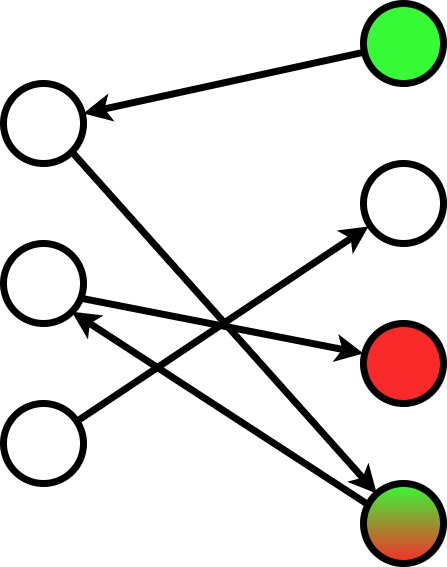
\includegraphics[width=0.10\textwidth, center]{content/various/matroid-intersection.jpg}
\end{center}

Let’s find the path from some green vertex to some red vertex. 
Objects on the path are added or removed from the set $S$, respectively, objects from the right part are added and the left part is removed.
